% Created by tikzDevice version 0.12.5 on 2023-10-08 01:39:54
% !TEX encoding = UTF-8 Unicode
\definecolor{color1}{HTML}{CC9966}
\definecolor{color2}{HTML}{99CCFF}
\definecolor{viridis0}{RGB}{255, 255, 255}
\definecolor{viridis1}{RGB}{253, 231, 37}
\definecolor{viridis2}{RGB}{181, 222, 43}
\definecolor{viridis3}{RGB}{110, 206, 88}
\definecolor{viridis4}{RGB}{53, 183, 121}
\definecolor{viridis5}{RGB}{31, 158, 137}
\definecolor{viridis6}{RGB}{38, 130, 142}
\definecolor{viridis7}{RGB}{49, 104, 142}
\definecolor{viridis8}{RGB}{62, 73, 137}
\definecolor{viridis9}{RGB}{72, 40, 120}
\definecolor{viridis10}{RGB}{68, 1, 84}
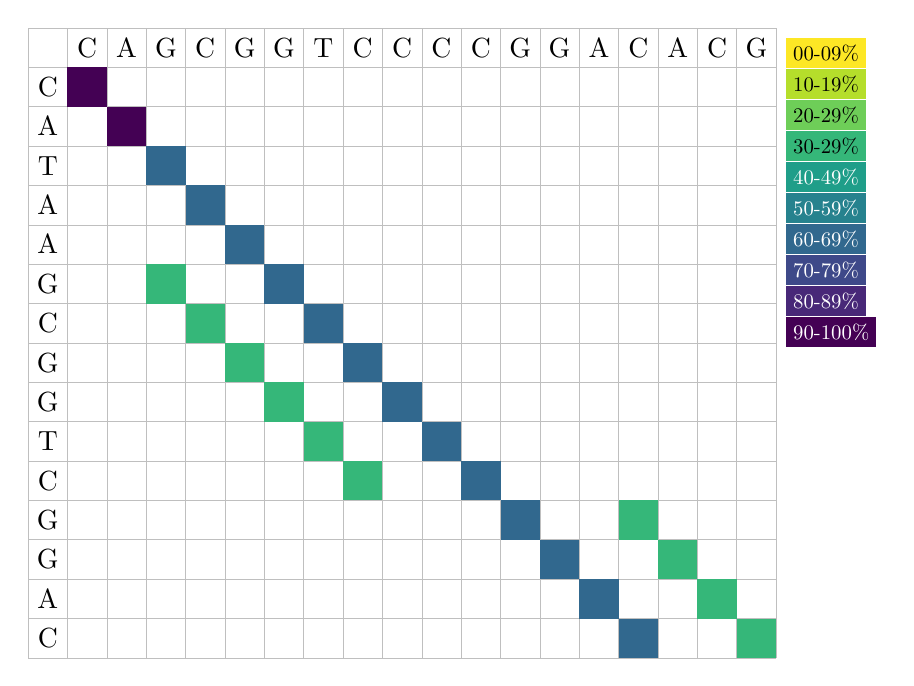
\begin{tikzpicture}[box/.style={rectangle, fill=gray!50, minimum size=0.5cm}]
\draw[very thin, color = gray!50, step = 0.5] (0,0) grid (9.5, 8);
\node at (0.25,7.25) {C};
\node at (0.25,6.75) {A};
\node at (0.25,6.25) {T};
\node at (0.25,5.75) {A};
\node at (0.25,5.25) {A};
\node at (0.25,4.75) {G};
\node at (0.25,4.25) {C};
\node at (0.25,3.75) {G};
\node at (0.25,3.25) {G};
\node at (0.25,2.75) {T};
\node at (0.25,2.25) {C};
\node at (0.25,1.75) {G};
\node at (0.25,1.25) {G};
\node at (0.25,0.75) {A};
\node at (0.25,0.25) {C};
\node at (0.75,7.75) {C};
\node at (1.25,7.75) {A};
\node at (1.75,7.75) {G};
\node at (2.25,7.75) {C};
\node at (2.75,7.75) {G};
\node at (3.25,7.75) {G};
\node at (3.75,7.75) {T};
\node at (4.25,7.75) {C};
\node at (4.75,7.75) {C};
\node at (5.25,7.75) {C};
\node at (5.75,7.75) {C};
\node at (6.25,7.75) {G};
\node at (6.75,7.75) {G};
\node at (7.25,7.75) {A};
\node at (7.75,7.75) {C};
\node at (8.25,7.75) {A};
\node at (8.75,7.75) {C};
\node at (9.25,7.75) {G};
\node[box, fill=viridis10] at (0.75, 7.25){};
\node[box, fill=viridis10] at (1.25, 6.75){};
\node[box, fill=viridis7] at (1.75, 6.25){};
\node[box, fill=viridis7] at (2.25, 5.75){};
\node[box, fill=viridis7] at (2.75, 5.25){};
\node[box, fill=viridis4] at (1.75, 4.75){};
\node[box, fill=viridis7] at (3.25, 4.75){};
\node[box, fill=viridis4] at (2.25, 4.25){};
\node[box, fill=viridis7] at (3.75, 4.25){};
\node[box, fill=viridis4] at (2.75, 3.75){};
\node[box, fill=viridis7] at (4.25, 3.75){};
\node[box, fill=viridis4] at (3.25, 3.25){};
\node[box, fill=viridis7] at (4.75, 3.25){};
\node[box, fill=viridis4] at (3.75, 2.75){};
\node[box, fill=viridis7] at (5.25, 2.75){};
\node[box, fill=viridis4] at (4.25, 2.25){};
\node[box, fill=viridis7] at (5.75, 2.25){};
\node[box, fill=viridis7] at (6.25, 1.75){};
\node[box, fill=viridis4] at (7.75, 1.75){};
\node[box, fill=viridis7] at (6.75, 1.25){};
\node[box, fill=viridis4] at (8.25, 1.25){};
\node[box, fill=viridis7] at (7.25, 0.75){};
\node[box, fill=viridis4] at (8.75, 0.75){};
\node[box, fill=viridis7] at (7.75, 0.25){};
\node[box, fill=viridis4] at (9.25, 0.25){};
\matrix [draw, below right, draw=none] at (current bounding box.north east) {
        % \node[box, fill=viridis0, scale=0.75] {0\%}; \\
        \node[box, fill=viridis1, scale=0.75] {00-09\%}; \\
        \node[box, fill=viridis2, scale=0.75] {10-19\%}; \\
        \node[box, fill=viridis3, scale=0.75] {20-29\%}; \\
        \node[box, fill=viridis4, scale=0.75] {30-29\%}; \\
        \node[box, fill=viridis5, scale=0.75] {\textcolor{white}{40-49\%}}; \\
        \node[box, fill=viridis6, scale=0.75] {\textcolor{white}{50-59\%}}; \\
        \node[box, fill=viridis7, scale=0.75] {\textcolor{white}{60-69\%}}; \\
        \node[box, fill=viridis8, scale=0.75] {\textcolor{white}{70-79\%}}; \\
        \node[box, fill=viridis9, scale=0.75] {\textcolor{white}{80-89\%}}; \\
        \node[box, fill=viridis10, scale=0.75] {\textcolor{white}{90-100\%}}; \\
    };
\end{tikzpicture}
